\documentclass[svgnames,11pt]{beamer}
\input{/home/tof/Documents/Cozy/latex-include/preambule_commun.tex}
\input{/home/tof/Documents/Cozy/latex-include/preambule_beamer.tex}
%\usepackage{pgfpages} \setbeameroption{show notes on second screen=left}
\author[]{Christophe Viroulaud}
\title{Représentation des entiers naturels}
\date{\framebox{\textbf{DonRep 01}}}
%\logo{}
\institute{Première - NSI}

\begin{document}
\begin{frame}
\titlepage
\end{frame}
\begin{frame}
    \frametitle{}

Un ordinateur n'interprète que des signaux électriques:
\begin{itemize}
    \item impulsion électrique $\rightarrow$ 1,
    \item pas d'impulsion $\rightarrow$ 0.
\end{itemize}
Nous parlons de \textbf{BInary DigiTS} ou plus simplement la contraction \textbf{bits}. 
\end{frame}
\begin{frame}
    \frametitle{}

    \begin{center}
        \begin{framed}
            Comment représenter les nombres entiers dans la mémoire de l'ordinateur?
        \end{framed}
    \end{center}

\end{frame}
\section{Cellules mémoires}
\begin{frame}
    \frametitle{Cellules mémoires}

    \begin{center}
        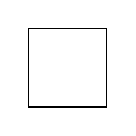
\begin{tikzpicture}
            \draw (0,0) grid (1,1);
        \end{tikzpicture}
        \captionof{figure}{Le bit est la plus petite unité informatique.}
    \end{center}

\end{frame}
\begin{frame}
    \frametitle{}

    \begin{center}
        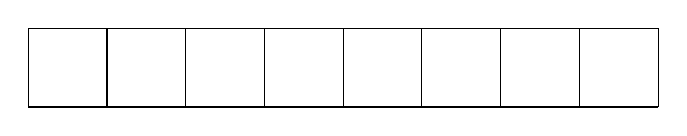
\begin{tikzpicture}
            \draw (0,0) grid (8,1);
        \end{tikzpicture}
        \captionof{figure}{8 bits représentent un \textbf{octet}.}
    \end{center}

\end{frame}
\begin{frame}
    \frametitle{}
\begin{aretenir}[]
Un ordinateur manipule des \textbf{mots mémoires} de 2, 4 ou 8 octets.
\end{aretenir}
    \begin{center}
        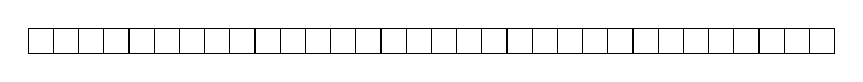
\begin{tikzpicture}[scale=0.32]
            \draw (0,0) grid (32,1);
        \end{tikzpicture}
        \captionof{figure}{Une machine \emph{32 bits} manipule des mots de 4 octets (4×8 = 32 bits) quand elle effectue des opérations.}
    \end{center}

\end{frame}
\begin{frame}
    \frametitle{}

    \begin{activite}
        Chaque bit accepte 2 valeurs possibles: 0 ou 1. Avec 1 bit nous pouvons donc avoir 2 combinaisons possibles.
        \begin{enumerate}
        \item Combien de combinaisons peut-on réaliser avec 1 octet?
        \item Même question pour 1 mot-mémoire 32 bits?
        \end{enumerate}
        \end{activite}

\end{frame}
\begin{frame}
    \frametitle{Correction}

    \begin{itemize}
        \item 1 octet $\rightarrow 2^8 = 256$ combinaisons.
        \item 1 mot 32 bits $\rightarrow 2^{32} = 4~294~967~296$ combinaisons.
    \end{itemize}
\note[item]{4 milliards}
\note[item]{PC récent = 64 bits}
\end{frame}
\section{Encodage des entiers naturels}
\subsection{Écriture en base 10}
\begin{frame}
    \frametitle{Écriture en base 10}

    $$6103 = 6×10^3 + 1×10^2 + 0×10^1 + 3×10^0$$


\end{frame}
\begin{frame}
    \frametitle{}

    \begin{activite}
        \begin{enumerate}
        \item Décomposer 76035 en base 10.
        \item Combien d'entiers en base 10 peut-on représenter avec 4 chiffres? Indiquer le plus petit et le plus grand.
        \item Combien d'entiers en base 10 peut-on représenter avec \emph{k} chiffres? Indiquer le plus petit et le plus grand.
        \end{enumerate}
        \end{activite}

\end{frame}
\begin{frame}
    \frametitle{Correction}

    \begin{itemize}
        \item Nous pouvons représenter $10^4$
        entiers avec 4 chiffres: de 0 à 9999.
        \item Nous pouvons représenter $10^k$
        entiers avec k chiffres: de 0 à $10^k−1$.
    \end{itemize}

\end{frame}
\subsection{Écriture en base 2}
\begin{frame}
    \frametitle{Écriture en base 2}
\note{Et si on avait que 2 doigts?}
    

    $$5 = 1×2^2 + 0×2^1 + 1×2^0$$
    $$5_{10}=101_2$$
    \begin{aretenir}[Remarque]
        Afin d'éviter les ambiguïtés, il est possible d'écrire un nombre en précisant sa base: $1001_2$.
    \end{aretenir}
\end{frame}
\begin{frame}
    \frametitle{}

    \begin{activite}
        \begin{enumerate}
        \item Calculer la valeur de l'entier représenté par le nombre binaire suivant: $101001_2$.
        \item Combien d'entiers peut-on représenter avec 8 chiffres binaires ? Indiquer le plus petit et le plus grand.
        \item Combien d'entiers peut-on représenter avec \emph{k} chiffres binaires? Indiquer le plus petit et le plus grand.
        \item Quel est le plus grand entier que l'on peut stocker dans un mot-mémoire 32 bits?
        \end{enumerate}
        \end{activite}

\end{frame}
\begin{frame}
    \frametitle{Correction}

    \begin{itemize}
        \item<1-> $1×2^5+0×2^4+1×2^3+0×2^2+0×2^1+1×2^0=41$
        \item<2-> Avec un octet nous pouvons représenter $2^8$ entiers: de 0 à 255
        \item<3-> Avec k chiffres nous pouvons représenter $2^k$ entiers: de 0 à $2^k−1$
        \item<4->$2^{32}-1=4294967295$
    \end{itemize}

\end{frame}
\subsection{Conversion}
\begin{frame}
    \frametitle{Conversion}
    Chaque entier est converti en base 2 avant d’être stocké en mémoire.
$$1×2^5+0×2^4+1×2^3+0×2^2+0×2^1+1×2^0=41$$
\begin{itemize}
    \item Dans 41 il y a \textbf{1} fois $2^5=32$
    \item Dans 9 ($41-32$) il y a \textbf{0} fois $2^4=16$
    \item Dans 9 il y a \textbf{1} fois $2^3=8$
    \item Dans 1 ($9-8$) il y a \textbf{0} fois $2^2=4$
    \item Dans 1 il y a \textbf{0} fois $2^1=2$
    \item Dans 1 il y a \textbf{1} fois $2^0=1$
\end{itemize}
    

\end{frame}
\begin{frame}
    \frametitle{Méthode équivalente}

    \begin{center}
        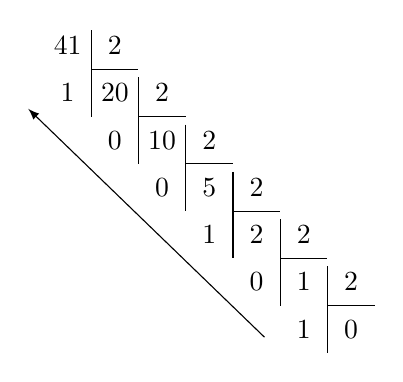
\begin{tikzpicture}
            \node at(0,0){41};
            \node at(0.6,0){2};
            \node at(0,-0.6){1};
            \node at(0.6,-0.6){20};
            \draw (0.3,0.2)--(0.3,-0.9);
            \draw (0.3,-0.3)--(0.9,-0.3);

            \node at(1.2,-0.6){2};
            \node at(0.6,-1.2){0};   
            \node at(1.2,-1.2){10};         
            \draw (0.9,-0.4)--(0.9,-1.5);
            \draw (0.9,-0.9)--(1.5,-0.9);

            \node at(1.8,-1.2){2};
            \node at(1.2,-1.8){0};   
            \node at(1.8,-1.8){5};         
            \draw (1.5,-1.0)--(1.5,-2.1);
            \draw (1.5,-1.5)--(2.1,-1.5);

            \node at(2.4,-1.8){2};
            \node at(1.8,-2.4){1};   
            \node at(2.4,-2.4){2};         
            \draw (2.1,-1.6)--(2.1,-2.7);
            \draw (2.1,-2.1)--(2.7,-2.1);

            \node at(3.0,-2.4){2};
            \node at(2.4,-3.0){0};   
            \node at(3.0,-3.0){1};         
            \draw (2.7,-2.2)--(2.7,-3.3);
            \draw (2.7,-2.7)--(3.3,-2.7);

            \node at(3.6,-3.0){2};
            \node at(3.0,-3.6){1};   
            \node at(3.6,-3.6){0};         
            \draw (3.3,-2.8)--(3.3,-3.9);
            \draw (3.3,-3.3)--(3.9,-3.3);
            \draw [->,>=latex] (2.5,-3.7) -- (-0.5,-0.8);
        \end{tikzpicture}
    \end{center}

\end{frame}
\begin{frame}
    \frametitle{}

    \begin{activite}
    Convertir $37_{10}$ en base 2.
    \end{activite}

\end{frame}
\begin{frame}
    \frametitle{Correction}

    \begin{center}
        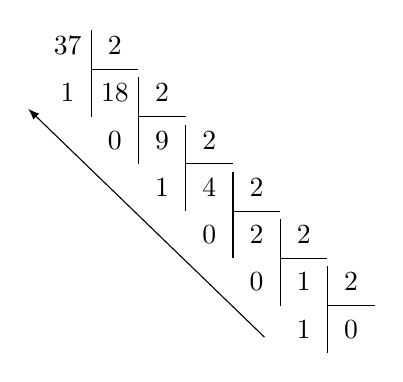
\begin{tikzpicture}
            \node at(0,0){37};
            \node at(0.6,0){2};
            \node at(0,-0.6){1};
            \node at(0.6,-0.6){18};
            \draw (0.3,0.2)--(0.3,-0.9);
            \draw (0.3,-0.3)--(0.9,-0.3);

            \node at(1.2,-0.6){2};
            \node at(0.6,-1.2){0};   
            \node at(1.2,-1.2){9};         
            \draw (0.9,-0.4)--(0.9,-1.5);
            \draw (0.9,-0.9)--(1.5,-0.9);

            \node at(1.8,-1.2){2};
            \node at(1.2,-1.8){1};   
            \node at(1.8,-1.8){4};         
            \draw (1.5,-1.0)--(1.5,-2.1);
            \draw (1.5,-1.5)--(2.1,-1.5);

            \node at(2.4,-1.8){2};
            \node at(1.8,-2.4){0};   
            \node at(2.4,-2.4){2};         
            \draw (2.1,-1.6)--(2.1,-2.7);
            \draw (2.1,-2.1)--(2.7,-2.1);

            \node at(3.0,-2.4){2};
            \node at(2.4,-3.0){0};   
            \node at(3.0,-3.0){1};         
            \draw (2.7,-2.2)--(2.7,-3.3);
            \draw (2.7,-2.7)--(3.3,-2.7);

            \node at(3.6,-3.0){2};
            \node at(3.0,-3.6){1};   
            \node at(3.6,-3.6){0};         
            \draw (3.3,-2.8)--(3.3,-3.9);
            \draw (3.3,-3.3)--(3.9,-3.3);
            \draw [->,>=latex] (2.5,-3.7) -- (-0.5,-0.8);
        \end{tikzpicture}
    \end{center}
$$37_{10}=100101_2$$
\end{frame}
\subsection{Écriture en base 16}
\begin{frame}
    \frametitle{Écriture en base 16}

    La base 16 est régulièrement utilisé pour représenter les nombres binaires plus facilement. Chaque chiffre hexadécimal est représenté par 4 bits.
    \begin{aretenir}[]
    1 octet est représenté par 2 chiffres hexadécimaux.
    \end{aretenir}

\end{frame}
\begin{frame}
    \frametitle{}

    \begin{activite}
        Compléter le tableau.
        \begin{center}{\small
            \begin{tabular}{|c|c|c|}
            \hline 
            décimal&hexadécimal & bits \\ 
            \hline 
            0&0 & 0000 \\ 
            \hline 
            1&1 & 0001 \\ 
            \hline 
            2&2 &  \\ 
            \hline 
            3&3 &  \\ 
            \hline 
            4&4 &  \\ 
            \hline 
            5&5 &  \\ 
            \hline 
            6&6 &  \\ 
            \hline 
            7&7 &  \\ 
            \hline 
            8&8 &  \\ 
            \hline 
            9&9 &  \\ 
            \hline 
            10&A &  \\ 
            \hline 
            11&B &  \\ 
            \hline 
            12&C &  \\ 
            \hline 
            13&D &  \\ 
            \hline 
            14&E &  \\ 
            \hline 
            15&F &  \\ 
            \hline 
            \end{tabular} }
            \end{center}
    \end{activite}

\end{frame}
\begin{frame}
    \frametitle{Correction}

    \begin{center}{\small
        \begin{tabular}{|c|c|c|}
        \hline 
        décimal&hexadécimal & bits \\ 
        \hline 
        0&0 & 0000 \\ 
        \hline 
        1&1 & 0001 \\ 
        \hline 
        2&2 & 0010 \\ 
        \hline 
        3&3 & 0011 \\ 
        \hline 
        4&4 & 0100 \\ 
        \hline 
        5&5 & 0101 \\ 
        \hline 
        6&6 & 0110 \\ 
        \hline 
        7&7 &  0111\\ 
        \hline 
        8&8 &  1000\\ 
        \hline 
        9&9 &  1001\\ 
        \hline 
        10&A & 1010 \\ 
        \hline 
        11&B & 1011 \\ 
        \hline 
        12&C &  1100\\ 
        \hline 
        13&D &  1101\\ 
        \hline 
        14&E &  1110\\ 
        \hline 
        15&F &  1111\\ 
        \hline 
        \end{tabular} }
        \end{center}

\end{frame}
\subsection{Python et les entiers}
\begin{frame}
    \frametitle{Python et les entiers}
\begin{itemize}
    \item<1-> Par défaut les nombres entiers sont encodés en base 10 en Python.
    \item<2-> Pour utiliser des nombres binaires, il suffit d'ajouter le préfixe \texttt{\textbf{0b}}.
    \item<3-> Le préfixe \texttt{\textbf{0x}} permet de manipuler des nombres en base hexadécimale.
    \item<4-> La fonction \texttt{\textbf{bin()}} convertit en base 2 n'importe quelle valeur.
\end{itemize}
\end{frame}
\begin{frame}
    \frametitle{}

    \begin{activite}
        Dans la console, écrire:
        \begin{enumerate}
        \item \textbf{\texttt{0b01001100}}
        \item \textbf{\texttt{0xAD2}}
        \item \textbf{\texttt{bin(76)}}
        \item Convertir le nombre binaire \texttt{\textbf{10101}} en décimal.
        \item Convertir le nombre hexadécimal \texttt{\textbf{F3A}} en base 2.
        \end{enumerate}
        \end{activite}

\end{frame}
\begin{frame}[fragile]
    \frametitle{Correction}

\begin{center}
\begin{lstlisting}[language=Python , basicstyle=\ttfamily\small, xleftmargin=2em, xrightmargin=2em]
>>> 0b01001100
76
>>> 0xAD2
2770
>>> bin(76)
'0b01001100'
>>> 0b10101
21
>>> bin(0xF3A)
'0b111100111010'
\end{lstlisting}
\end{center}

\end{frame}
\end{document}